\documentclass[A4,12PT, english, twocolumn]{journal}
\usepackage{amsmath,amssymb,amsfonts}
\usepackage[margin=0.7in]{geometry}
\usepackage{graphicx}
\usepackage{enumitem}
\usepackage{xcolor}
\usepackage{hyperref}
\usepackage{tabularray}
\usepackage{multicol}
\usepackage{tikz}
\usepackage{circuitikz}
\usepackage{scalerel}
\usepackage{pict2e}
\usepackage{tkz-euclide}
\usetikzlibrary{calc}
\usetikzlibrary{patterns,arrows.meta}
\usetikzlibrary{shadows}
\usetikzlibrary{external}

%pgfplots
\usepackage{pgfplots}
\pgfplotsset{compat=newest}
\usepgfplotslibrary{statistics}
\usepgfplotslibrary{fillbetween}

\def\infinity{\rotatebox{90}{8}}

% Hiperlink
\hypersetup{
    colorlinks=true,
    linkcolor=blue,
    filecolor=magenta,      
    urlcolor=cyan,
    pdftitle={Overleaf Example},
    pdfpagemode=FullScreen,
}
%\usepackage{style}
\NewDocumentCommand{\Log}{o}{%
\IfNoValueTF{#1}{}{{}^{#1}\!}\log}%
  
%command buat logaritma dengan basisnya di pojok kiri
%\textheight=17cm
%\textwidth=10cm
%\usepackage{blindtext}
\setenumerate[1]{itemsep=0,5cm}
\setenumerate[2]{topsep=5pt, itemsep=5pt, label=\textbf{\Alph*}.}

\title{Matematika Saintek \& Fisika UTUL UGM 2017 Kode 814}
\author{Fauzan Akbar Sukandar Putra \\ \LaTeX}

\begin{document}
\maketitle

%\begin{minipage}{0.5\textwidth}
\begin{enumerate}

%1%
\item $\lim\limits_{x \longrightarrow -y}\dfrac{\tan{x} + \tan{y}}{\left( \frac{x^2 - y^2}{-2y^2} \right) \left( 1 - \tan{x}\tan{y} \right)}=$\dots
    \begin{enumerate}
        \item $-1$
        \item $1$
        \item $0$
        \item $y$
        \item $-y$
    \end{enumerate}

%2%
\item Jika $f(x) = b^x, \; b$ konstanta positif, maka $\frac{f \left( x^2 -1 \right)}{f \left( 1-x^2 \right)}=$\dots
    \begin{enumerate}
        \item $f(1 - x^2)f(x^2 - 1)$
        \item $f(1 - x^2)f(x^2 - 1)$
        \item $f(x^2 - 1)f(  x^2 - 1)$
        \item $f(1 - x^2) + f(1 - x^2)$
        \item $f(x^2 - 1) + f(  x^2 - 1)$
    \end{enumerate}

%3%
\item DIberikan garis lurus melalui $(0,-2)$ dan $\left( \frac{3}{2} , 0 \right)$. Jarak parabola $ y = x^2 - 1 $ ke garis tersebut adalah\dots
	\begin{enumerate}
       \item $\frac{5}{6}$ 
       \item $\frac{2}{3}$    
       \item $\frac{1}{2}$ 
       \item $\frac{1}{3}$   
       \item $\frac{1}{6}$
	\end{enumerate}

%4%
\item Diberikan dua vektor $\vec{u} = (1, -1, 2)$ dan $\vec{v} = (-1,1,-1)$ . Jika vektor $\vec{w}$ mempunyai panjang satu dan tegak lurus dengan vektor $\vec{u}$ dan $\vec{v}$, maka $\vec{w} =$\dots
	\begin{enumerate}
       \item $(0,0,0)$
       \item $\left( \frac{1}{2}\sqrt{2}, \frac{1}{2}\sqrt{2}, 0 \right)$
       \item $\left( \frac{1}{2}\sqrt{2}, -\frac{1}{2}\sqrt{2}, 0   \right)$
       \item $\left( -\frac{2}{3}, \frac{1}{3}, \frac{2}{3} \right)$
       \item $ \left( \frac{2}{3} , \frac{1}{3}, \frac{2}{3} \right)$
	\end{enumerate}  

%5%
\item Diketahui suatu deret tak hingga $\sin 2x \sin ^2x + \sin 2x \sin ^4 x + \sin 2x \sin ^6 x + ...$, $ 0 < x \leq \frac{\pi}{4} $. Nilai maksimum deret tak hingga tersebut adalah\dots
	\begin{enumerate}
       \item $32$ 
       \item $16$   
       \item $8$ 
       \item $4$   
       \item $1$ 
	\end{enumerate}

%6%
\item Diketahui vektor-vektor $\vec{u} = a\vec{i}+\vec{j}+2\vec{k}$ dan $\vec{v} = -\vec{i}-\vec{j}-\vec{k}$. Jika vektor $\vec{w}$ tegak lurus vektor $\vec{u}$ dan $\vec{v}$ dengan panjang vektor $\vec{w}$ adalah $3$, maka jumlah nilai-nilai $a$ yang memenuhi adalah\dots
	\begin{enumerate}
       \item $0$ 
       \item $1$   
       \item $3$ 
       \item $4$   
       \item $5$
	\end{enumerate}  

%7%
\item Banyak bilangan tiga digit yang berbeda yang disusun dari angka $0,1,2,...,9$ dan habis dibagi oleh $5$ adalah\dots
	\begin{enumerate}
       \item $136$ 
       \item $144$   
       \item $128$  
       \item $162$    
       \item $180$
	\end{enumerate}

%8%
\item Jika salah satu akar persamaan $x^3 + 2x^2 + px - 6 = 0$ adalah $2$, maka jumlah dua akar lainnya adalah\dots
	\begin{enumerate}
       \item $-4$  
       \item $-2$    
       \item $1$  
       \item $2$     
       \item $6$
	\end{enumerate}

%9%
\item Jika $f\left( \frac{2x+1}{x-3} \right) = x^2 + 2x - 3$, maka nilai dari $f^\prime (0)$ adalah\dots
	\begin{enumerate}
       \item $-2\frac{1}{4}$ 
       \item $-2$   
       \item $-1\frac{3}{4}$ 
       \item $-1\frac{1}{4}$   
       \item $-1$
	\end{enumerate}

%10%
\item Diketahui kubus $ABCD.EFGH$ dengan panjang rusuk $4 \; cm$. Jarak titik $C$ ke bidang $BDG$ adalah\dots
	\begin{enumerate}
       \item $\frac{4}{3}\sqrt{3}$ 
       \item $\frac{3}{4}\sqrt{3}$  
       \item $\frac{4}{3}\sqrt{2}$ 
       \item $\frac{3}{4}\sqrt{2}$   
       \item $\frac{8}{3}$
	\end{enumerate}

%11%
\item Diketahui dua bilangan real positif $x$ dan $y$. Jika $x + 2y = 20$, maka nilai maksimum dari $x^2y$ adalah\dots
	\begin{enumerate}
       \item $\frac{16000}{9}$ 
       \item $\frac{16000}{27}$  
       \item $\frac{4000}{27}$ 
       \item $\frac{1600}{27}$   
       \item $\frac{400}{9}$
	\end{enumerate}

%12% 
\item Jika $\tan{A} = \frac{4}{3}$, dan $\tan {B} = 7$, maka $A + B =$\dots
	\begin{enumerate}
       \item $45^\circ$ 
       \item $135^\circ$   
       \item $150^\circ$ 
       \item $225^\circ$  
       \item $330^\circ$
	\end{enumerate}

%13%
\item DIberikan bilangan-bilangan positif $x_1$ dan $x_2$. Jika $12, x_1, x_2$ membentuk barisan aritmetika dan $x_1, x_2, 4$ membentuk barisan geometri, maka $x_1 + x_2 =$\dots
	\begin{enumerate}
       \item $6$  
       \item $8$   
       \item $10$  
       \item $13$  
       \item $15$
	\end{enumerate}

%14%    
\item Persamaan lingkaran yang melalui perpotongan dua lingkaran $L_1 \equiv x^2+y^2 - 2x - 2y - 2 = 0$ dan $L_2 \equiv x^2+y^2 + 2x - 6y +6 = 0$ serta berpusat di garis $g \equiv x - 2y = 5$ adalah\dots
	\begin{enumerate}
       \item $x^2 + y^2 - 6x + 2y - 5 = 0$
       \item $x^2 + y^2 - 6x + 2y - 10 = 0$ 
       \item $x^2 + y^2 + 6x + 8y - 5 = 0$
       \item $x^2 + y^2 + 6x + 8y - 10 = 0$ 
       \item $x^2 + y^2 + 6x + 8y  = 0$
	\end{enumerate}

%15%
\item Semua nilai $x$ yang memenuhi $|x|+|x-2| > 3$ adalah\dots
	\begin{enumerate}
       \item $x < -1$ atau $x > \frac{5}{2}$
       \item $x < -\frac{1}{2}$ atau $x > 3$
       \item $x < -\frac{1}{2}$ atau $x > \frac{5}{2}$
       \item $x < -1$ atau $ x > 3$
       \item $x < -\frac{3}{2}$ atau $x > \frac{5}{2}$
	\end{enumerate}

    
%FISIKA %
%16%
\newpage
\item Pada planet $A$ yang berbentuk bola dibuat terowongan lurus dari permukaan planet $A$ yang menembus pusat planet dan berujung di permukaan planet $A$ pada tempat terjauh dari pangkal terowongan. Selanjutnya dihitung waktu yang dibutuhkan dari sebuah partikel untuk  bergerak dari pangkal menuju ujung terowongan di planet $A$. Terowongan sejenis juga dibuat di planet $B$ yang sama-sama berbentuk bola dimana planet $B$ memiliki rapat massa rata-rata yang sama dengan rapat massa rata-rata planet $A$ namun jari-jari planet $B$ dua kali jari-jari planet $A$. Perbandingan waktu tempuh di dalam terowongan $A$ dan $B$ adalah\dots
    \begin{enumerate}
        \item $1:1$
        \item $1:\sqrt{2}$
        \item $1:2$
        \item $1:2\sqrt{2}$
        \item $1:4$
    \end{enumerate}
  
%17%
\item Grafik yang menunjukkan bahwa benda diperlambat dengan perlambatan konstan adalah\dots
    \begin{enumerate}
        \item 
            \begin{tikzpicture}[baseline]
                \draw[thick, red] (0,2.5) -- (5,2.5);
                \draw[thick, ->] (0,0) -- (5,0) node[right=1pt]{\Large $t$};
                \draw[thick, ->] (0,0) -- (0,5) node[above=1pt]{\Large $v$};
            \end{tikzpicture}
        \item 
            \begin{tikzpicture}[baseline]
                \draw[thick, red] (0,1) -- (5,5);
                \draw[thick, ->] (0,0) -- (5,0) node[right=1pt]{\Large $t$};
                \draw[thick, ->] (0,0) -- (0,5) node[above=1pt]{\Large $v$};
            \end{tikzpicture}
        \item 
            \begin{tikzpicture}[baseline]
                \draw[thick, red] (0,4) -- (5,1);
                \draw[thick, ->] (0,0) -- (5,0) node[right=1pt]{\Large $t$};
                \draw[thick, ->] (0,0) -- (0,5) node[above=1pt]{\Large $v$};
            \end{tikzpicture}
        \item 
            \begin{tikzpicture}[baseline]
                \draw[thick, red] (0,1) -- (2.5,4) -- (5,1);
                \draw[thick, ->] (0,0) -- (5,0) node[right=1pt]{\Large $t$};
                \draw[thick, ->] (0,0) -- (0,5) node[above=1pt]{\Large $v$};
            \end{tikzpicture}
        \item 
            \begin{tikzpicture}[baseline]
                \draw[thick, red] (2.5,1) parabola (1,5);
                \draw[thick, red] (2.5,1) parabola (4,5);
                \draw[thick, ->] (0,0) -- (5,0) node[right=1pt]{\Large $t$};
                \draw[thick, ->] (0,0) -- (0,5) node[above=1pt]{\Large $v$};
            \end{tikzpicture}  
    \end{enumerate}
     
%18%
\item Sebuah batu dilemparkan ke atas dari permukaan tanah dengan kecepatan $v_0$. Selang waktu $t$ kemudian, batu kedua dilemparkan ke atas dari permukaan tanah. Ternyata batu kedua sampai ke tanah dalam waktu $t$ sebelum batu pertama sampai ke tanah. Jika percepatan gravitasi adalah $g$ maka selisih tinggi maksimum kedua batu adalah\dots
    \begin{enumerate}
        \item $\frac{1}{2}t (gt-2v_0)$
        \item $\frac{1}{2}t (gt-v_0)$
        \item $\frac{1}{2}t (2v_0+gt)$
        \item $t(2v_0+gt)$
        \item $t(2v_0-gt)$
    \end{enumerate}
   
%19% 
\item Sebuah benda dilemparkan ke atas dari ketinggian $7 \; m$ dengan kecepatan awal $2 \; m/s$. Jika $g= 10 \; m/s^2$, maka lama benda di udara adalah\dots
    \begin{enumerate}
        \item $1 \; detik$
        \item $1,2 \; detik$
        \item $1,4 \; detik$
        \item $1,6 \; detik$
        \item $2 \; detik$
    \end{enumerate}

%20%
\item Sebuah peluru bermassa $m_1$ ditembakkan dengan kelajuan $v$ ke dalam bandul balistik bermassa $m_2$. Carilah katinggian maksimum yang dicapai bandul jika peluru menembus bandul dan muncul dengan kelajuan $\frac{v}{2}$.
    \begin{enumerate}
        \item $\frac{m_1^2 v^2}{8gm_2^2}$
        \item $\frac{m_2^2 v^2}{8gm_1^2}$
        \item $\frac{m_1 m_2 v^2}{8gm_2^2}$
        \item $\frac{m_1 m_2 v^2}{8gm_1^2}$
        \item $\frac{m_2^2 v^2}{8g m_1 m_2}$
    \end{enumerate}

%21%
\item Lima buah massa $M$ yang sama berjarak pisah sama pada busur sebuah setengah lingkaran berjari-jari $R$ sebagaimana ditunjukkan pada gambar. Sebuah massa $m$ diletakkan di pusat kelengkungan busur tersebut. Jika $M$ adalah $3 \; kg, \; m$ adalah $2 \; kg,$ dan $R= 10 \; cm$. Berapakah gaya pada $m$ yang disebabkan oleh kelima massa tersebut?
\begin{center}
    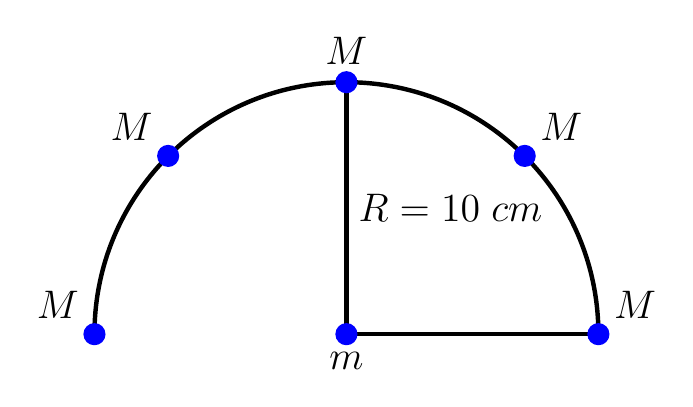
\begin{tikzpicture}[scale=0.8]
        %GRID
        %\draw[lightgray] (0,0) grid (10,10);
        
        %KOORDINAT
        \coordinate (A) at (8,0);
        \coordinate (B) at (4,4);
        \coordinate (C) at (0,0);
        \coordinate (D) at (4,0);
        \coordinate (E) at (6.83,2.83);
        \coordinate (F) at (1.17,2.83);
        
        %BUSUR
        \draw[ultra thick] (0,0) arc (180:0:4cm);

        \draw[ultra thick] (8,0) -- (4,0) -- node[midway, right=0.01cm]{\Large $R=10 \; cm$} (4,4);
        
        %LINGKARAN
        \fill[blue] (A) circle (5pt) node[black, above right=3pt]{\Large $M$};
        \fill[blue] (B) circle (5pt) node[black, above=3pt]{\Large $M$};
        \fill[blue] (C) circle (5pt) node[black, above left=3pt]{\Large $M$};
        \fill[blue] (D) circle (5pt) node[black, below=3pt]{\Large $m$};
        \fill[blue] (E) circle (5pt) node[black, above right=3pt]{\Large $M$};
        \fill[blue] (F) circle (5pt) node[black, above left=3pt]{\Large $M$};
    \end{tikzpicture}
\end{center}
    \begin{enumerate}
        \item $1,22 \times 10^{-8} \; N$
        \item $3,28 \times 10^{-8} \; N$
        \item $4,8 \times 10^{-8} \; N$
        \item $7,6 \times 10^{-8} \; N$
        \item $9,66 \times 10^{-8} \; N$
    \end{enumerate}
    
%22% 
\item $N$ buah balok dengan massa yang sama di atas lantai yang licin disusun seperti pada gambar.
\begin{center}
    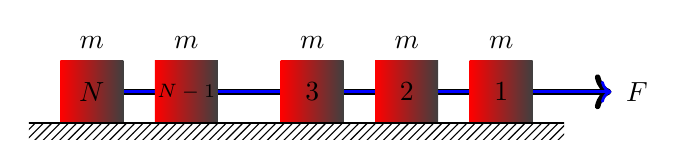
\begin{tikzpicture}[scale=0.4]
    %GRID
    % \draw[lightgray] (0,0) grid (10,5);

    5TALI
    \draw[line width=2pt, ->] (0,1) -- (16.5,1) node[right=1pt]{$F$};
    \draw[line width=1pt, ->, color=blue] (0,1) -- (16.5,1);
    
    %KOTAK2
    \shade[left color=red, right color=darkgray] (-1,0) rectangle node[midway]{$N$} (1,2) node[midway, above=12pt]{$m$};
    
    \shade[left color=red, right color=darkgray] (2,0) rectangle node[midway]{\scriptsize $N-1$} (4,2) node[midway, above=12pt]{$m$};
    
    \shade[left color=red, right color=darkgray] (6,0) rectangle node[midway]{$3$} (8,2) node[midway, above=12pt]{$m$};
    
    \shade[left color=red, right color=darkgray] (9,0) rectangle node[midway]{$2$} (11,2) node[midway, above=12pt]{$m$};
    
    \shade[left color=red, right color=darkgray] (12,0) rectangle node[midway]{$1$} (14,2) node[midway, above=12pt]{$m$};

    %LANTAI
    \fill[pattern=north east lines] (-2,-0.5) rectangle (15,0);
    \draw[thick] (-2,0) rectangle (15,0);
    
    \end{tikzpicture}
\end{center}
Balok yang paling kanan ditarik dengan gaya $F$ ke kanan. Besarnya tegangan tali antara balok $2$ dan $3$ adalah\dots
    \begin{enumerate}
        \item $\frac{N-2}{N}F$
        \item $\frac{N-3}{N-1}F$
        \item $\frac{N-1}{N}F$
        \item $\frac{N-3}{N}F$
        \item $\frac{N-2}{N-1}F$
    \end{enumerate}
    
%23%
\item Sebuah silinder homogen bermassa $M$ berjari-jari $R$ menggelinding tanpa slip turun dari ketinggian $h$ pada sebuah bidang miring dengan sudut kemiringan $\alpha$. Momentum sudut silinder terhadap sumbu pusat massanya setelah mencapai dasar bidang miring adalah\dots
    \begin{enumerate}
        \item $4MR \sqrt{\frac{gh}{2}}$
        \item $MR \sqrt{\frac{gh}{3}}$
        \item $3MR \sqrt{\frac{gh}{4}}$
        \item $MR \sqrt{\frac{gh}{5}}$
        \item $2MR \sqrt{\frac{gh}{6}}$
    \end{enumerate}
    
%24%  
\item Pernyataan berikut ini yang salah untuk benda yang mengalami gerak harmonik sederhana adalah\dots
	\begin{enumerate}
		\item Pada saat simpangan benda $= \frac{1}{2}$ simpangan maksimum, energi potensialnya $= \frac{1}{2}$ energi potensial maksimum.
		\item Saat di titik setimbang, energi kinetiknya maksimum.
		\item Pada saat di titik terjauh, energi kinetiknya nol.
		\item Arah percepatan benda selalu berlawanan dengan arah simpangan.
		\item Jumlah energi kinetik dan energi potensial selalu tetap.
	\end{enumerate}
	
%25%
\item Bahwa gelombang cahaya tidak mungkin longitudinal dapat dipahami dari gejala\dots
   \begin{enumerate}
        \item Interferensi
        \item Difraksi
        \item Pemantulan
        \item Pembiasan
        \item Polarisasi
   \end{enumerate}
   
%26%
\item Sebuah elektron memasuki daerah yang mengandung medan magnet $B$ dan medan listrik $E$, dengan kecepatan awal $v$. Besar usaha yang dilakukan gaya magnet pada elektron ini adalah\dots
    \begin{enumerate}
        \item nol
        \item Sebanding dengan $v$
        \item Sebanding dengan $E \times B$
        \item Sama dengan energi potensial listriknya
        \item Sebanding dengan perubahan energi kinetiknya
    \end{enumerate}
  
%27%  
\item Perhatikan rangkaian listrik seperti ditunukkan pada gambar. Berapakah arus yang mengalir pada hambatan $2 \; \Omega$?
\begin{center}
    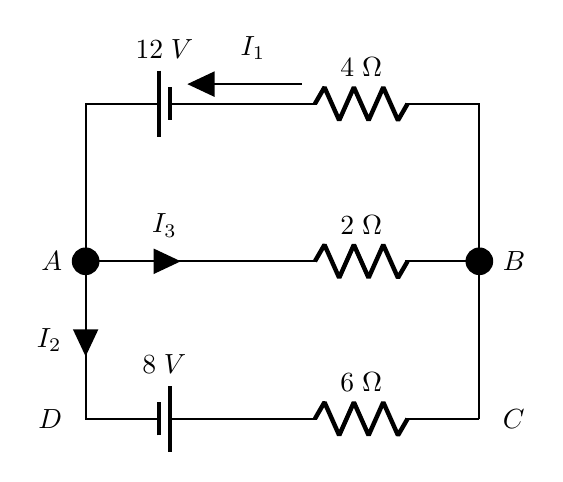
\begin{tikzpicture}
        %GRID
        %\draw[lightgray] (0,0) grid (5,5);

        %RANGKAIAN
        \draw[thick] (5,0) to[resistor, a=$6 \; \Omega$] (2,0) to[battery1, a=$8 \; V$] (0,0) -- node[currarrow, sloped, pos=0.5, scale=2, xscale=-1]{} node[midway, left=5pt]{$I_2$} (0,2);
        \draw[thick] (0,2) -- (0,4) to[battery1, a^=$12 \; V$] (2,4) to[resistor, a^=$4 \; \Omega$] (5,4) -- (5,0);

        \draw[thick] (0,2) -- node[currarrow, sloped, xscale=1, pos=0.5, scale=2]{} node[midway, above=5pt]{$I_3$} (2,2) to[resistor, a^=$2 \; \Omega$] (5,2);

        \draw[thick] (1.5,4.25) -- node[currarrow, sloped, pos=0, scale=2, xscale=-1]{} node[midway, above=5pt]{$I_1$} (2.75,4.25);

        %LINGKARAN
        \fill[black] (0,2) circle (5pt) node[left=5pt]{$A$};
        \fill[black] (5,2) circle (5pt) node[right=5pt]{$B$};
        \fill[black] (5,0) circle (0pt) node[right=5pt]{$C$};
        \fill[black] (0,0) circle (0pt) node[left=5pt]{$D$};
    \end{tikzpicture}
\end{center}
    \begin{enumerate}
        \item $91 \; A$
        \item $9,1 \; A$
        \item $0,91 \; A$
        \item $84 \; A$
        \item $8,4 \; A$
    \end{enumerate}
    
%28%  
\item Gambar berikut menunjukkan sebuah kubus, dimana sebuah muatan mula-mula berada pada titik asal $O$. Kubus tersebut diberi medan magnet homogen searah sumbu $y$. Jika muatan bergerak dengan kecepatan $v$ dengan arah sebagaimana ditunjukkan dengan anak panah berlabel angka $1,2,3,4,$ dan $5,$ tunjukkan pada arah dengan label angka nomor berapakah gaya  magnetik lenyap.
\begin{center}
    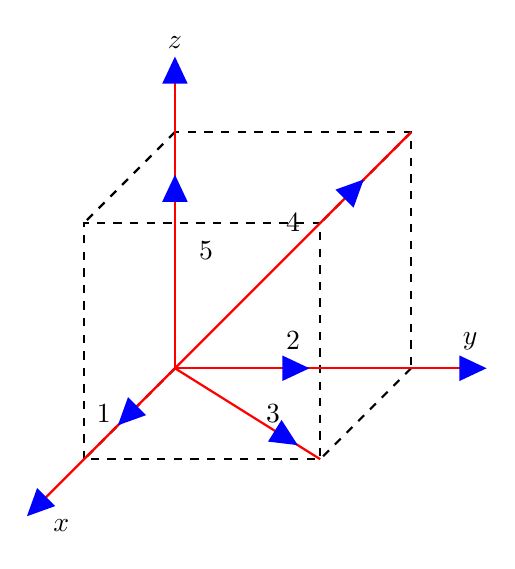
\begin{tikzpicture}[scale=3]
        
        %KUBUS
        \draw[black, thick, dashed] (0,0,0) -- (0,1,0) -- (1,1,0) -- (1,0,0) -- cycle;
        \draw[black, thick, dashed] (0,0,1) -- (0,1,1) -- (1,1,1) -- (1,0,1) -- cycle;
        \draw[black, thick, dashed] (0,0,0) -- (0,0,1);
        \draw[black, thick, dashed] (0,1,0) -- (0,1,1);
        \draw[black, thick, dashed] (1,1,0) -- (1,1,1);
        \draw[black, thick, dashed] (1,0,0) -- (1,0,1);

        %GARIS PANAH
        \draw[thick, red] (0,0,0) -- node[currarrow, sloped, scale=2, xscale=1, pos=0.5, blue]{} node[black, midway, above=3pt]{$2$} (1,0,0) -- (1.25,0,0) node[currarrow, sloped, scale=2, xscale=1, pos=1, blue]{} node[black, above=3pt]{$y$};

        \draw[thick, red] (0,0,0) -- node[blue, currarrow, sloped, scale=2, pos=0.5, xscale=-1]{} node[left=3pt, black]{$1$} (0,0,1) -- node[blue, currarrow, sloped, scale=2, pos=1, xscale=-1]{} node[black, below=10pt]{$x$} (0,0,1.5);

        \draw[thick, red] (0,0,0) --node[currarrow, pos=0.75, sloped, scale=2, xscale=1, blue]{} node[right=3pt, black]{$3$} (1,0,1);

        \draw[thick, red] (0,0,0) -- node[currarrow, sloped, scale=2, xscale=1, pos=0.75, blue]{} node[midway, right=25pt, above=3pt, black]{$4$} (1,1,0);

        \draw[thick, red] (0,0,0) -- node[currarrow, sloped, scale=2, xscale=1, pos=0.75, blue]{} node[black, above=20pt, right=5pt]{$5$} (0,1,0) -- (0,1.25,0) node[currarrow, sloped, scale=2, xscale=1, pos=1, blue]{} node[black, above=5pt]{$z$};
        
        %LABEL
        % \node[above] at (0,1,1) {A};
        % \node[right] at (1,1,1) {B};
        % \node[below] at (1,0,1) {C};
        % \node[left] at (0,0,1) {D};
        % \node[above] at (0,1,0) {E};
        % \node[right] at (1,1,0) {F};
        % \node[below] at (1,0,0) {G};
        % \node[left] at (0,0,0) {H};
    \end{tikzpicture}
\end{center}
    \begin{enumerate}
        \item $1$
        \item $2$
        \item $3$
        \item $4$
        \item $5$
    \end{enumerate}

%29%  
\item Sebuah kubus dengan koefisien muai panjang $\alpha$ mula-mula memiliki volume $V_0$. Setelah dipanaskan, pertambahan luasnya adalah $\Delta A$. Kenaikan suhu kubus adalah\dots
    \begin{enumerate}
        \item $\frac{1}{16}\Delta AV_0^{-\frac{2}{3}}\alpha^{-1}$
        \item $\frac{1}{12}\Delta AV_0^{-\frac{2}{3}}\alpha^{-1}$
        \item $\frac{1}{8}\Delta AV_0^{-\frac{2}{3}}\alpha^{-1}$
        \item $\frac{1}{6}\Delta AV_0^{-\frac{2}{3}}\alpha^{-1}$
        \item $\frac{1}{4}\Delta AV_0^{-\frac{2}{3}}\alpha^{-1}$
    \end{enumerate}

%30%
\item Suatu fenomena pada saat Big Bang dapat diwakili oleh konstanta alam fundamental yang dirumuskan sebagai $\sqrt{\frac{hc}{2\pi G}}$. Besaran ini berdimensi\dots
    \begin{enumerate}
        \item Massa
        \item Panjang
        \item Waktu
        \item Kecepatan
        \item Gaya
    \end{enumerate}

%31%
\item Suatu unsur antara $X$ memiliki waktu hidup $\tau$. Jika energi unsur itu diukur dan hasil pengukuran adalah $E$, maka ketidakpastian pengukuran itu adalah\dots
    \begin{enumerate}
        \item $\Delta E = E - \frac{h}{\tau}$
        \item $\Delta E = E + \frac{h}{\tau}$
        \item $\Delta E = \frac{h}{\tau}$
        \item $\Delta E = \frac{E^2 \tau}{h}$
        \item $\Delta E = \frac{h^2}{\tau^2 E}$
    \end{enumerate}

%32%
\item Dua pesawat bergerak secara relativistik menjauhi pengamat di bumi dengan kelajuan yang sama nauun arahnya berlawanan. Jika besarnya kecepatan relatif antar pesawat hanya $1,5$ kali kelajuan kedua pesawat menurut pengamat di bumi, maka besar kecepatan relatif antar pesawat tersebut adalah\dots
    \begin{enumerate}
        \item $\frac{1}{2}c$
        \item $\frac{2}{3}c$
        \item $\frac{1}{2}\sqrt{2}c$
        \item $\frac{1}{2}\sqrt{3}c$
        \item $\frac{1}{3}\sqrt{3}c$
    \end{enumerate}

%33%
\item Dalam eksperimen efek fotolistrik, potensial yang dibutuhkan untuk menghentikan elektron-elektron yang lepas\dots
    \begin{enumerate}
        \item Sama untuk semua intensitas berkas cahaya yang digunakan.
        \item Semakin tinggi jika intensitas berkas cahaya yang digunakan semakin tinggi.
        \item Semakin tinggi jika panjang gelombang cahaya yang digunakan semakin besar.
        \item Sama untuk berbagai frekuensi cahaya yang digunakan.
        \item Semakin rendah jika intensitas berkas cahaya yang digunakan semakin tinggi.
    \end{enumerate}

%34%
\item Sebuah partikel yang bergerak secara relativistik berkurang kecepatannya sedemikian sehingga energi total relativistiknya menjadi $75\%$ energi total relativistik mula-mula, serta energi kinetiknya relativistiknya menjadi $37,5\%$ energi kinetik relativistik mula-mula. Perbandingan antara momentum relativistik akhir dengan momentum relativistik awal adalah\dots
    \begin{enumerate}
        \item $\frac{9}{64}$
        \item $\frac{3}{8}$
        \item $\frac{9}{16}$
        \item $\frac{3}{5}$
        \item $\frac{3}{4}$
    \end{enumerate}

%35%
\item Sebuah elips memiliki setengah sumbu panjang $a$ dan setengah sumbu pendek $b$ jika diukur dalam keadaan diam. Seorang pengamat bergerak sepanjang garis lurus yang sejajar bidang elips dan sejajar sumbu panjang dengan kecepatan $v$. Luas elips itu menurut pengamat yang bergerak adalah\dots
    \begin{enumerate}
        \item $\pi a b$
        \item $\pi a b \sqrt{1-\left( \frac{v}{c} \right)^2}$
        \item $\pi a b \left( 1-\left( \frac{v}{c} \right)^2 \right)$
        \item $\pi a b \left( 1-\left( \frac{v}{c} \right)^2 \right)^{-\frac{1}{2}}$
        \item $\pi a b \left( 1-\left( \frac{v}{c} \right)^2 \right)^{-1}$
    \end{enumerate}

\end{enumerate}
\end{document}  
